\Chapter{Étude de plasmas magnétisés}
\chaptermark{Étude de plasmas magnétisés}
\begin{refsection}
Ce quatrième chapitre porte sur l'étude de deux cas concrets
chacun représentatif d'une configuration magnétique particulière : le filtre
magnétique avec le propulseur PEGASES et la colonne de plasma magnétisée de la
source d'ions négatifs CYBELE. 
A travers ces exemples, nous testons les possibilités du nouveau code MAGNIS,
tout en explorant la physique qu'il révèle. Les simulations sont discutées et
confrontées aux mesures expérimentales ainsi qu'aux résultats de modèles
statistiques.
En fin de chapitre, nous simulons une configuration typique de bord de tokamak,
de champ magnétique intense et où le transport est principalement de nature
turbulente. 
		 
\section{Barrière magnétique - PEGASES}
a

\begin{figure}[htbp]
\centering
\includegraphics[width=0.8\textwidth]{figures/4-pegases3D.png}
{\caption{Schéma de principe de fonctiopnnement du propulseur PEGASES avec les
différents étages mentionnés en italiques\parencite{Popelier}.}
\label{4-pegasesSimDomain}}
\end{figure}

a

\begin{figure}[htbp]
\centering
\includegraphics[width=0.6\textwidth]{figures/4-pegasesSimDomain.png}
{\caption{Le domaine de simulation est le plan perpendiculaire au champ
magnétique.}
\label{4-pegasesSimDomain}}
\end{figure}

a

\begin{figure}[htbp]
    \centering
    \subfigure[]{\label{4-PegasesCarteDensiteBase}
    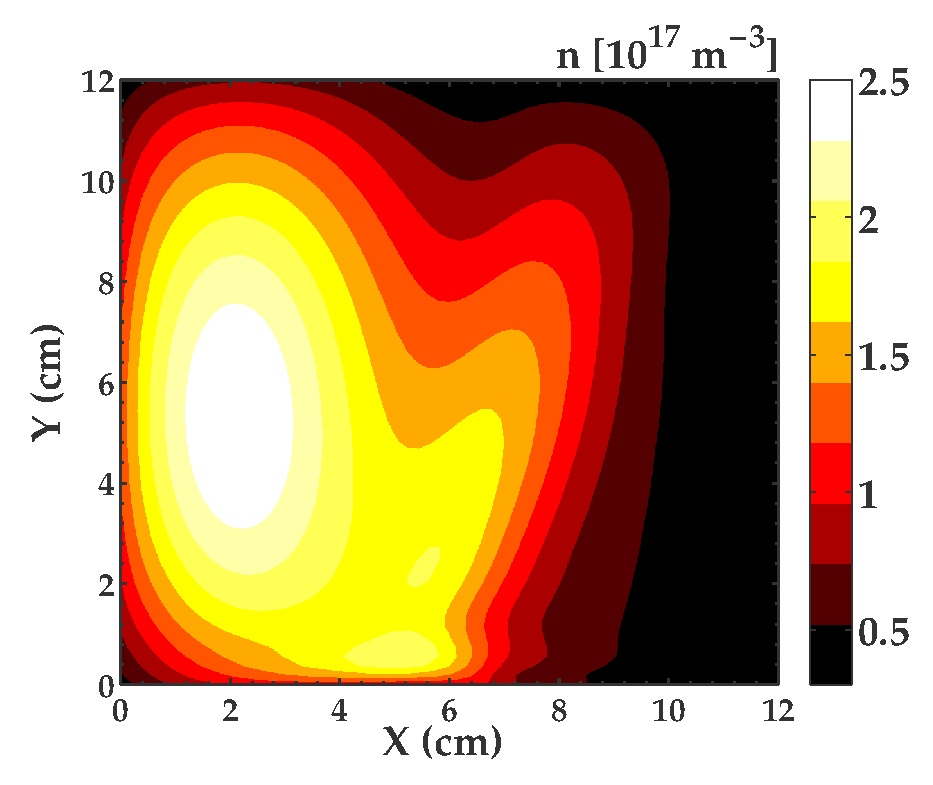
\includegraphics[height=5.75cm]{figures/4-PegasesCarteDensiteBase.eps}}
    \subfigure[]{\label{4-PegasesCartePotentielBase}
    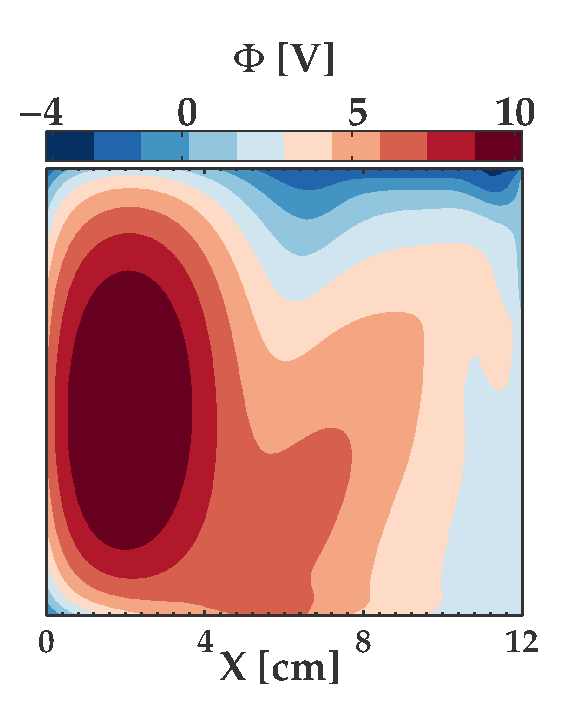
\includegraphics[height=5.75cm]{figures/4-PegasesCartePotentielBase.eps}}
    \subfigure[]{\label{4-PegasesCarteTemperatureBase}
    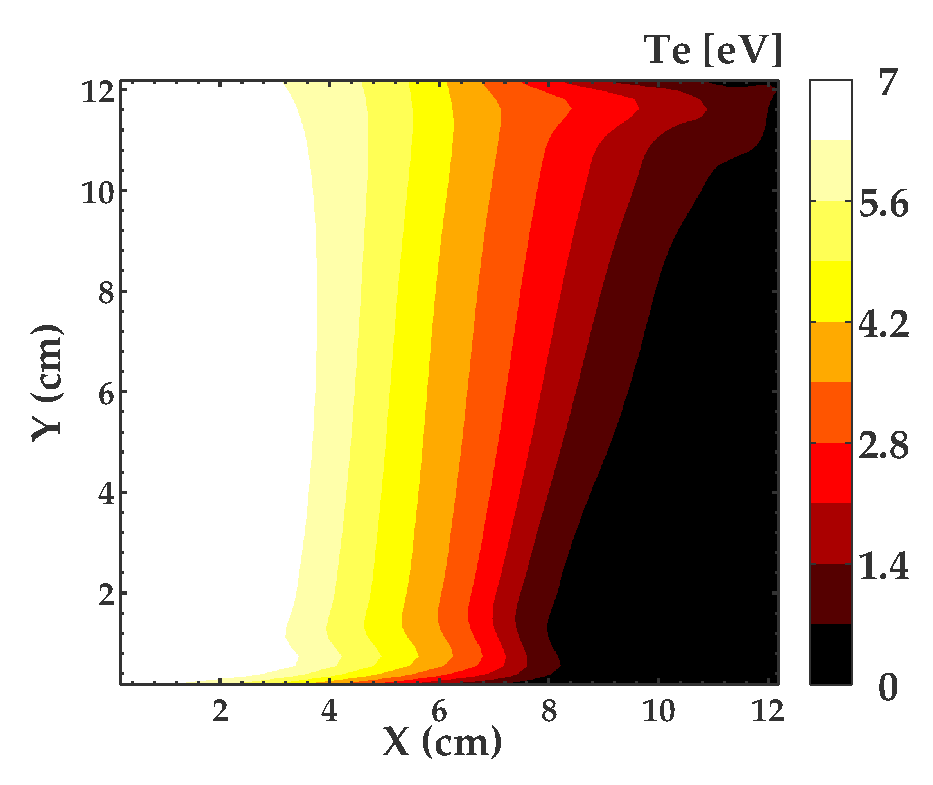
\includegraphics[height=5.75cm]{figures/4-PegasesCarteTemperatureBase.eps}}
    \caption{Cartes de densité \subref{4-PegasesCarteDensiteBase}, de potentiel
    \subref{4-PegasesCartePotentielBase} et de température \subref{4-PegasesCarteTemperatureBase}}
    \label{2-CartesWithTe}
	\end{figure}

a

\begin{figure}[htbp]
  \centering
    \subfigure[]{\label{4-PegasesCarteFluxEBase}
    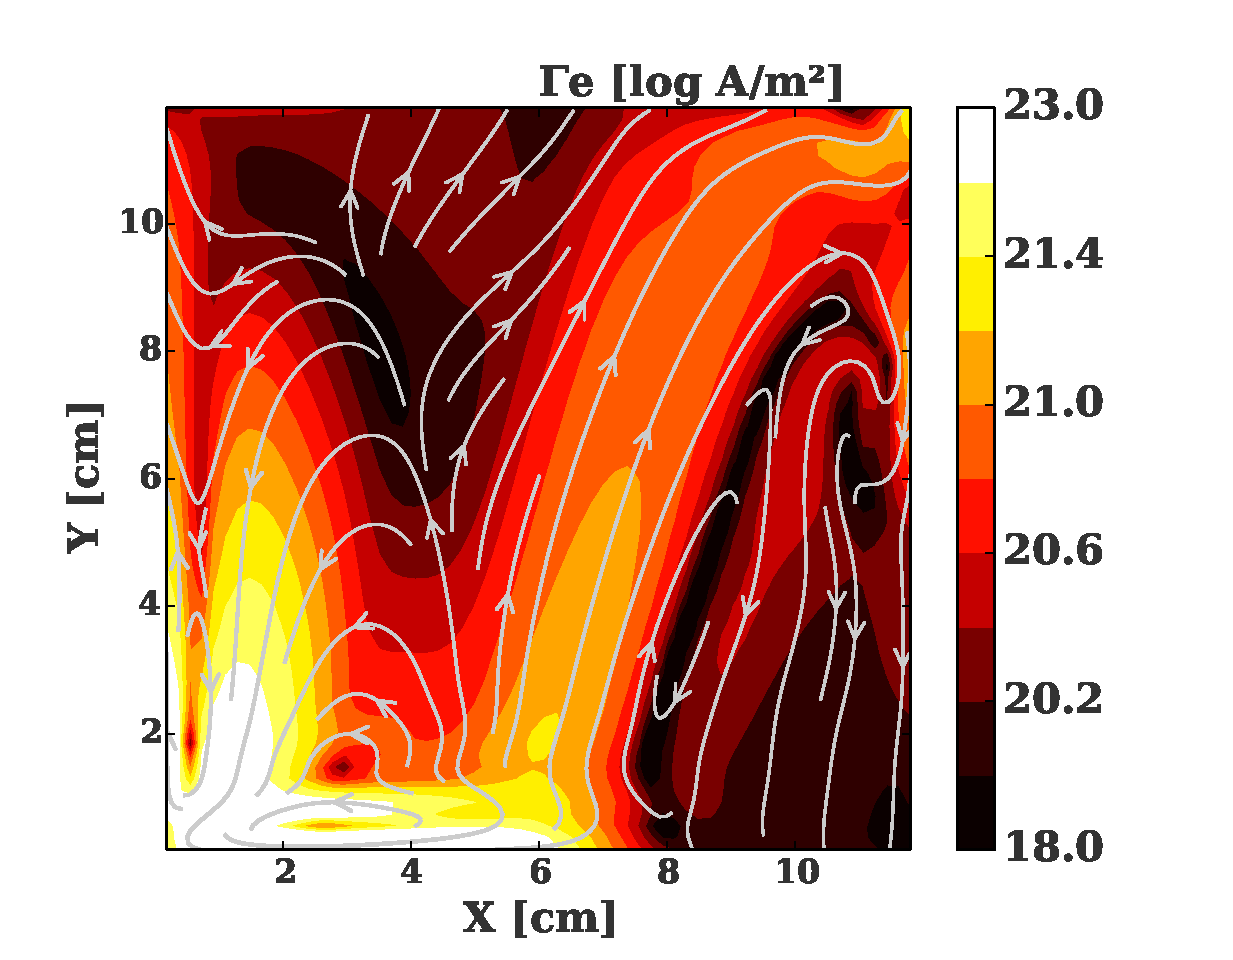
\includegraphics[height=4cm]{figures/4-PegasesCarteFluxEBase.eps}}
    \subfigure[]{\label{4-PegasesCarteFluxIBase}
    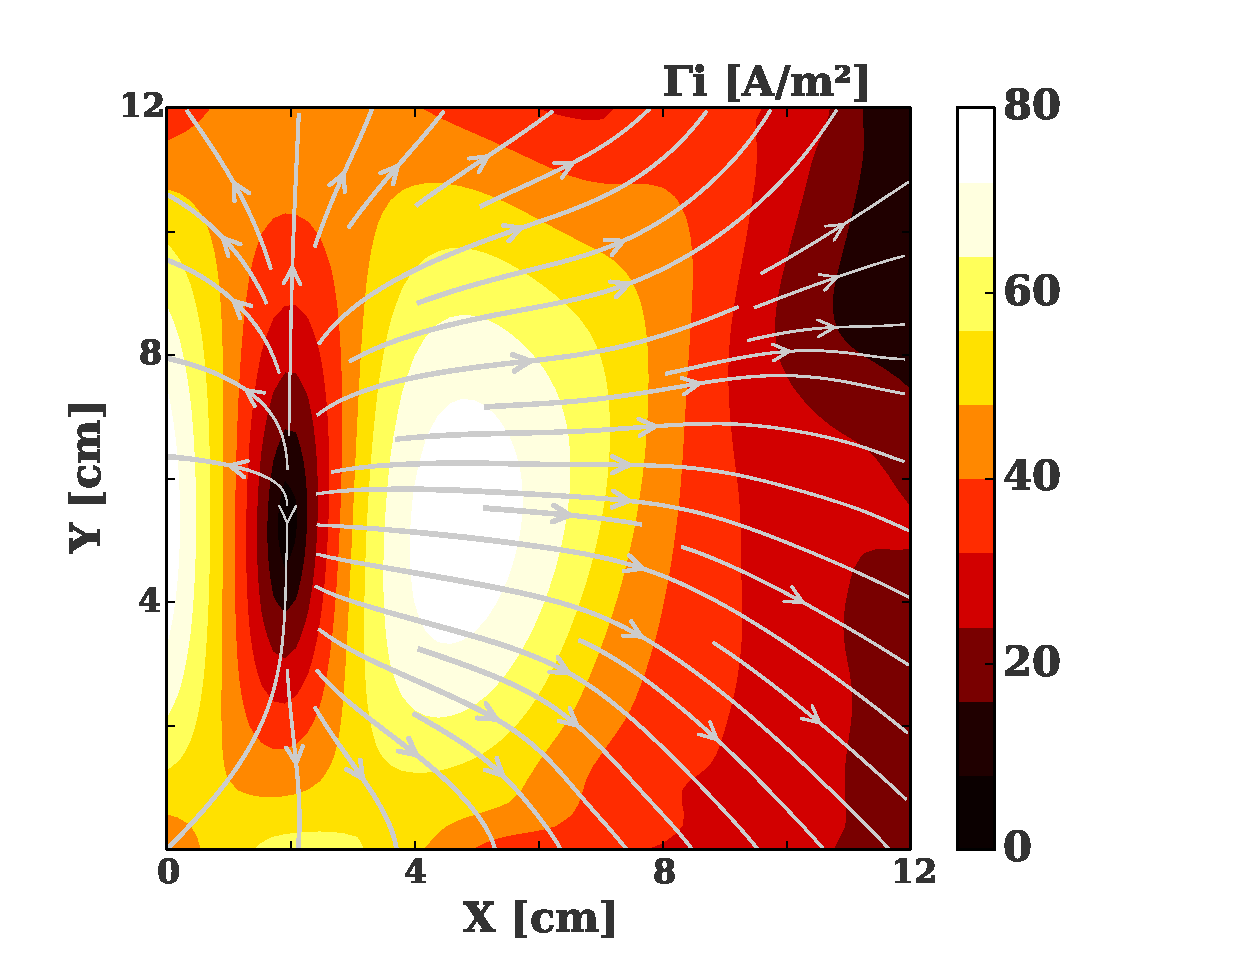
\includegraphics[height=4cm]{figures/4-PegasesCarteFluxIBase.eps}}
    \caption{Cartes de densité\subref{4-PegasesCarteFluxEBase}~, de
    potentiel\subref{4-PegasesCarteFluxEBase}~ et de
    température\subref{4-PegasesCarteFluxEBase}}
    \label{pandas}
\end{figure}
\subsection{Comparaison expérimentale}

a
	
	\subsubsection{Scan en pression}
	\begin{figure}[htbp]
  \centering
    \subfigure[]{\label{4-pegasesCompPressDenProfile}
    
\includegraphics[height=4cm]{figures/4-pegasesCompPressDenProfile.eps}}
    \subfigure[]{\label{4-pegasesCompPressTempProfile}
    
\includegraphics[height=4cm]{figures/4-pegasesCompPressTempProfile.eps}}
    \caption{Cartes de densité\subref{4-pegasesCompPressTempProfile}~, de
    potentiel\subref{4-pegasesCompPressTempProfile}~ et de
    température\subref{4-pegasesCompPressTempProfile}}
    \label{pandas}
\end{figure}
	\subsubsection{Variations du champ magnétique}

a
	
	\begin{figure}[htbp]
  \centering
    \subfigure[]{\label{4-pegasesCompMagDenProfile}
    
\includegraphics[height=4cm]{figures/4-pegasesCompMagDenProfile.eps}}
    \subfigure[]{\label{4-pegasesCompMagTempProfile}
    
\includegraphics[height=4cm]{figures/4-pegasesCompMagTempProfile.eps}}
    \caption{Cartes de densité\subref{4-pegasesCompMagTempProfile}~, de
    potentiel\subref{4-pegasesCompMagTempProfile}~ et de
    température\subref{4-pegasesCompMagTempProfile}}
    \label{pandas}
\end{figure}
\subsection{Transport du courant dans le cas de parois conductrices}

a
	
	\subsubsection{Influence du champ magnétique}
	a
	
\begin{figure}[htbp]
	\centering
	
\includegraphics[width=0.6\textwidth]{figures/4-pegasesVarMagCourantParoi.eps}
	{\caption{Courant total récupéré à la paroi en fonction de l'intensité du
	filtre magnétique pour trois voltages appliqués. }
	\label{pegasesVarMagCourantParoi}}
	\end{figure}
	
	a
	
	\subsubsection{Transport à travers le filtre magnétique}
	a
	
	\begin{figure}[htbp]
	\centering
	\includegraphics[width=0.85\textwidth]{figures/4-pegasesfluxElectronique.pdf}
	{\caption{Flux électronique à travers le filtre magnétique sur un plage
	allant de 0 à 500 Gauss pour trois différents voltages appliqués.}
	\label{4-pegasesfluxElectronique}}
	\end{figure}
\subsection{Phénomènes intermittents, instabilités}
	\subsubsection{Vagues ioniques}
	a
	
	\begin{figure}[htbp]
  \centering
    \subfigure[]{\label{4-PegasesCarteDensiteVarBias1}
    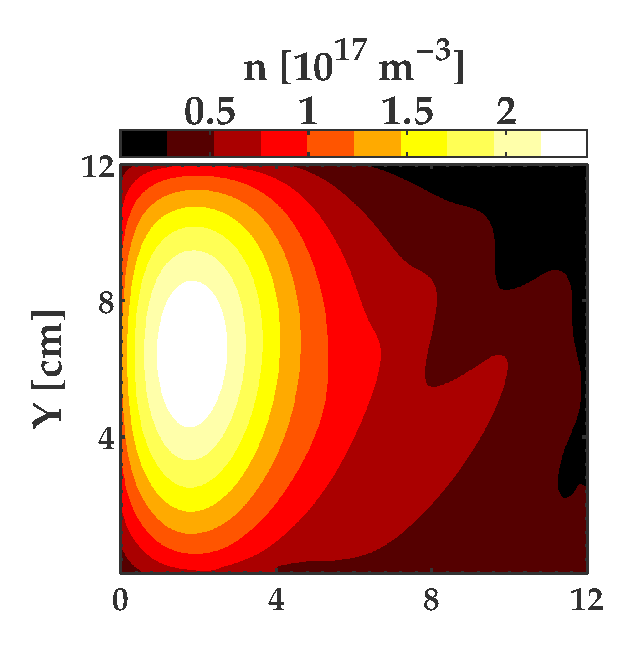
\includegraphics[height=6cm]{figures/4-PegasesCarteDensiteVarBias1.eps}}
    \subfigure[]{\label{4-PegasesCarteDensiteVarBias2}
    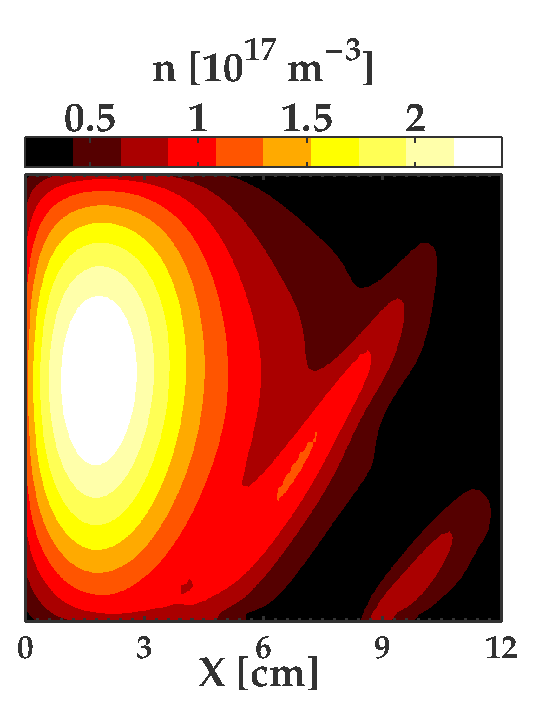
\includegraphics[height=6cm]{figures/4-PegasesCarteDensiteVarBias2.eps}}
    \subfigure[]{\label{4-PegasesCarteDensiteVarBias3}
    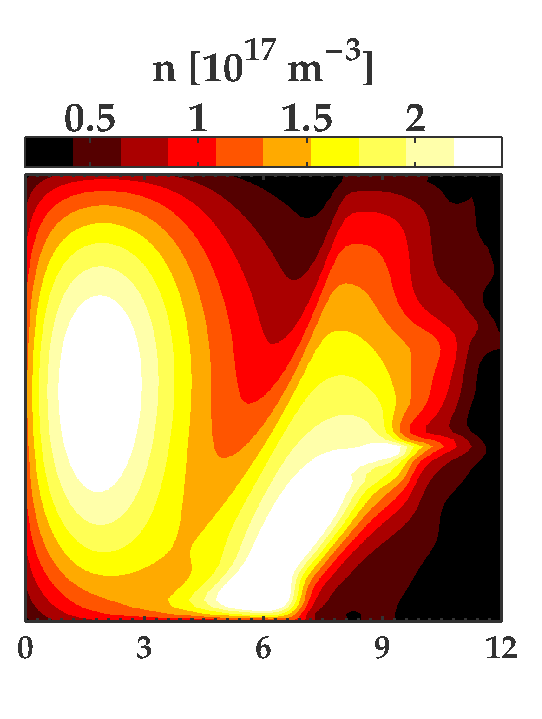
\includegraphics[height=6cm]{figures/4-PegasesCarteDensiteVarBias3.eps}}
    \caption{Cartes de densité\subref{4-PegasesCarteDensiteVarBias1}~, de
    potentiel\subref{4-PegasesCarteDensiteVarBias2}~ et de
    température\subref{4-PegasesCarteDensiteVarBias3}}
    \label{pandas}
\end{figure}

a

\begin{figure}[htbp]
  \centering
    \subfigure[]{\label{4-PegasesCarteDensiteVarBias4}
    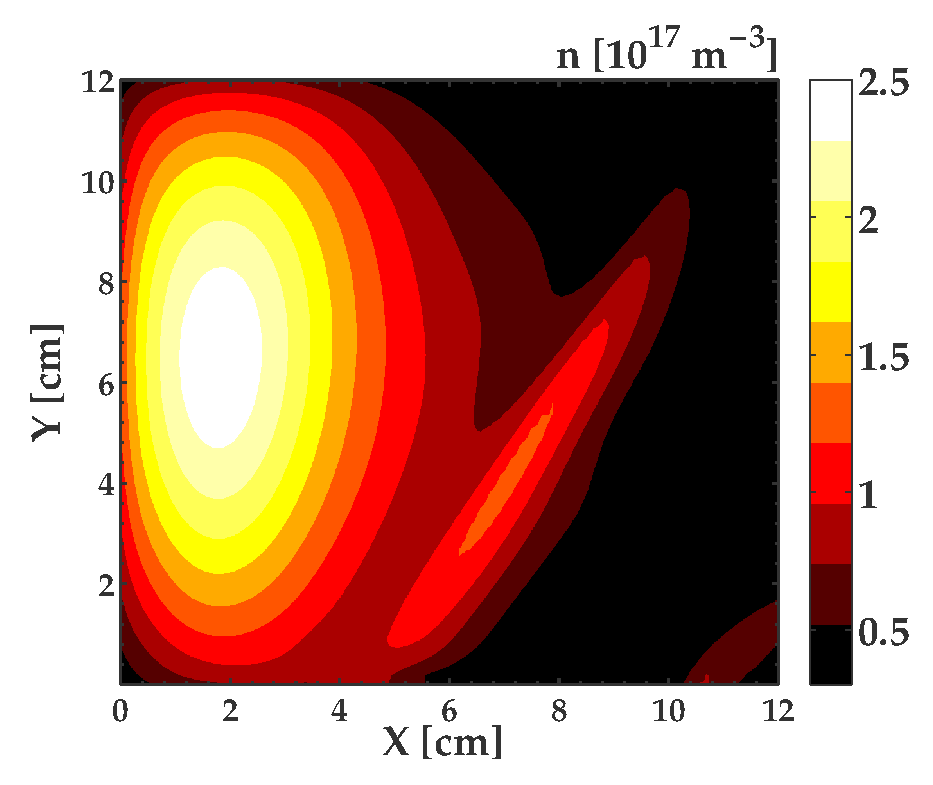
\includegraphics[height=5cm]{figures/4-PegasesCarteDensiteVarBias4.eps}}
    \subfigure[]{\label{4-PegasesCarteViSurTeVarBias}
    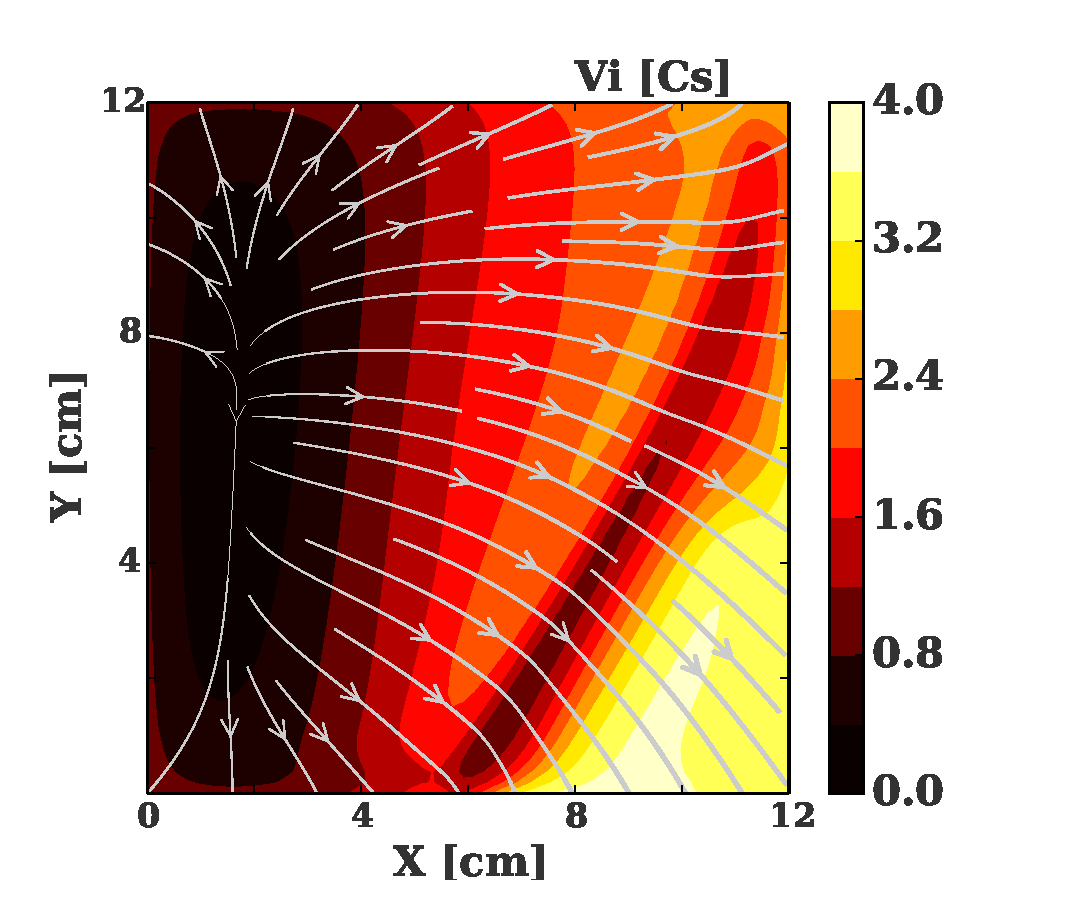
\includegraphics[height=5cm]{figures/4-PegasesCarteViSurTeVarBias.eps}}
    \caption{Cartes de densité\subref{4-PegasesCarteDensiteVarBias1}~, de
    potentiel\subref{4-PegasesCarteDensiteVarBias2}}
    \label{pandas}
\end{figure}
	
	a
	
	\subsubsection{Instabilité liée au gradient de densité}
	\begin{figure}[htbp]
  \centering
    \subfigure[]{\label{4-PegasesCarteDensiteVarBias5}
    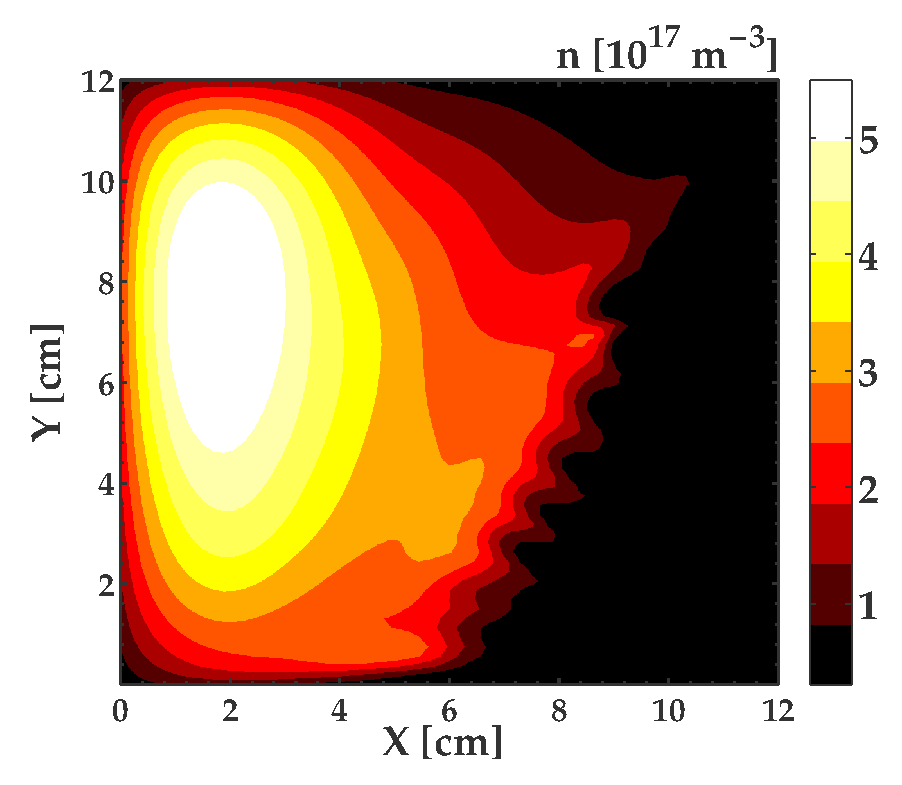
\includegraphics[height=5cm]{figures/4-PegasesCarteDensiteVarBias5.eps}}
    \subfigure[]{\label{4-PegasesCarteViSurTeVarBias6}
    \includegraphics[height=5cm]{figures/4-PegasesCarteViSurTeVarBias6.eps}}
    \caption{Cartes de densité\subref{4-PegasesCarteDensiteVarBias5}~, de
    potentiel\subref{4-PegasesCarteDensiteVarBias6}}
    \label{pandas}
\end{figure}
	
\section{Colonne de plasma magnétisée - CYBELE}
a

\begin{figure}[htbp]
  \centering
    \subfigure[]{\label{4-cybelePhoto}
    \includegraphics[height=12cm]{figures/4-cybelePhoto.png}}
    \subfigure[]{\label{4-cybeleSchema}
    \includegraphics[height=10cm]{figures/4-cybeleSchema.png}}
    \caption{Cartes de densité\subref{4-cybelePhoto}~, de
    potentiel\subref{4-cybeleSchema}}
    \label{pandas}
\end{figure}	

a

\begin{figure}[htbp]
\centering
\includegraphics[width=0.8\textwidth]{figures/4-magnetizedColumn.jpg}
{\caption{Transport des ions et des électrons dans une colonne de
plasma\parencite{Rozhansky}.}
\label{4-magnetizedColumn}}
\end{figure}

a

\begin{figure}[htbp]
\centering
\includegraphics[width=0.8\textwidth]{figures/4-cybeleSimDomain.png}
{\caption{Le domaine de simulation est le plan perpendiculaire au champ
magnétique.}
\label{4-cybeleSimDomain}}
\end{figure}

a

\begin{figure}[htbp]
  \centering
    \subfigure[]{\label{4-CybeleCarteDensiteBase}
    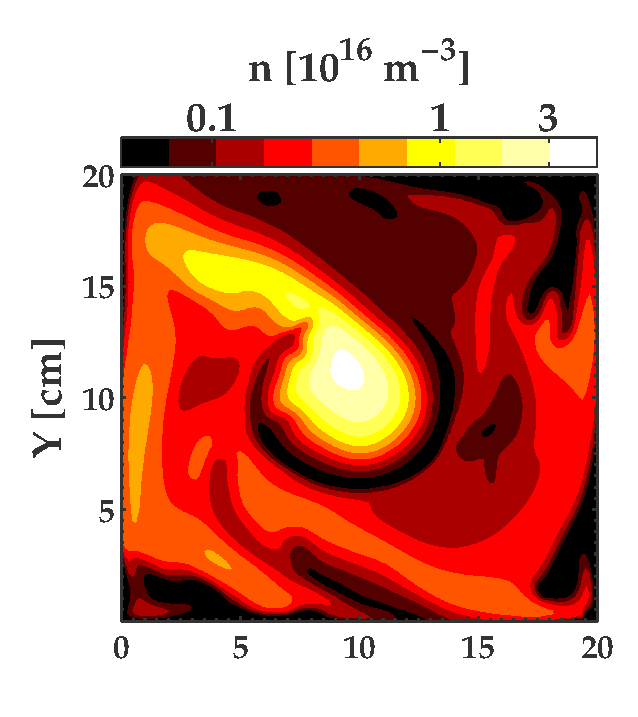
\includegraphics[height=5.5cm]{figures/4-CybeleCarteDensiteBase.eps}}
    \subfigure[]{\label{4-CybeleCartePotentielBase}
    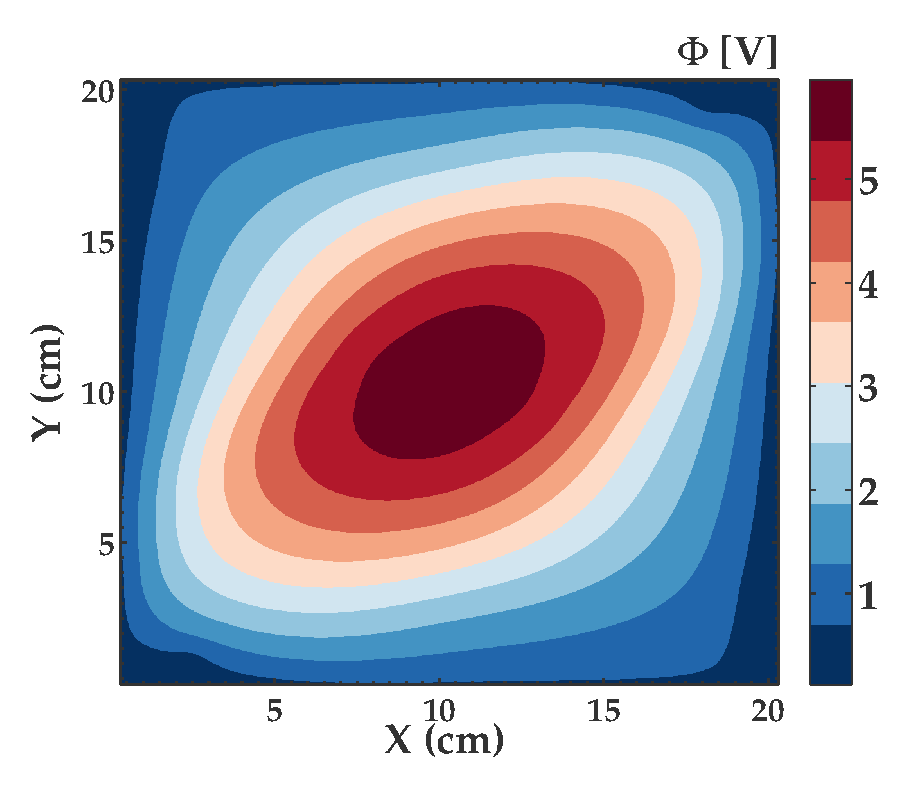
\includegraphics[height=5.5cm]{figures/4-CybeleCartePotentielBase.eps}}
    \subfigure[]{\label{4-CybeleCarteTemperatureBase}
    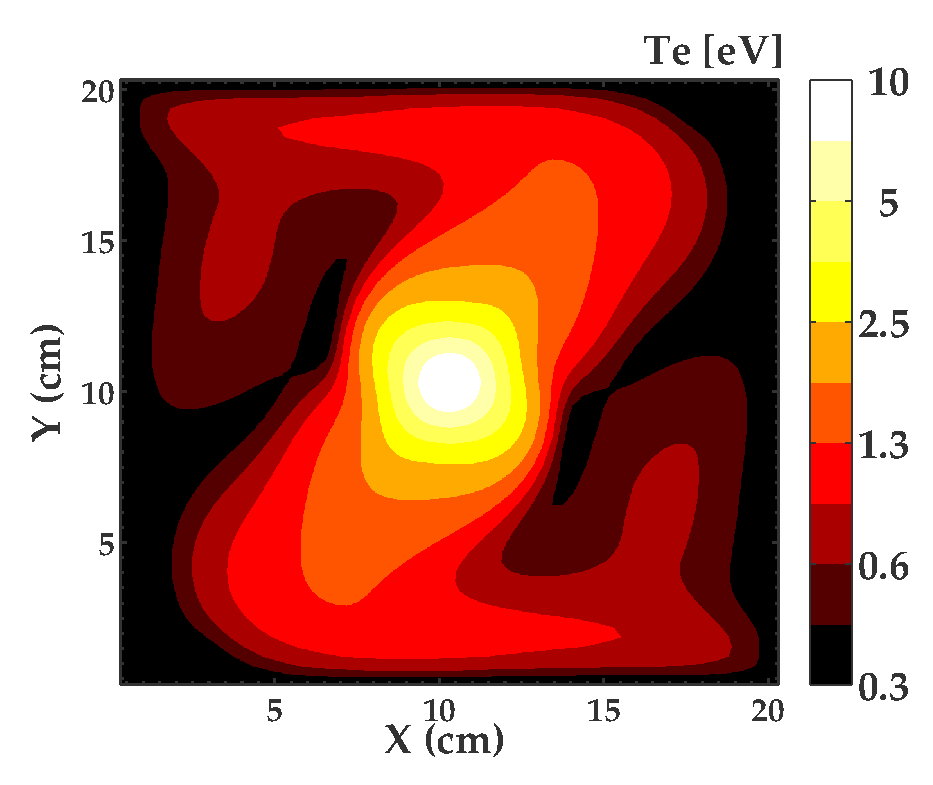
\includegraphics[height=5.5cm]{figures/4-CybeleCarteTemperatureBase.eps}}
    \caption{Cartes de densité \subref{4-CybeleCarteDensiteBase}~, de
    potentiel \subref{4-CybeleCartePotentielBase}~ et de
    température \subref{4-CybeleCarteTemperatureBase}}
    \label{pandas}
\end{figure}

a

\begin{figure}[htbp]
\centering
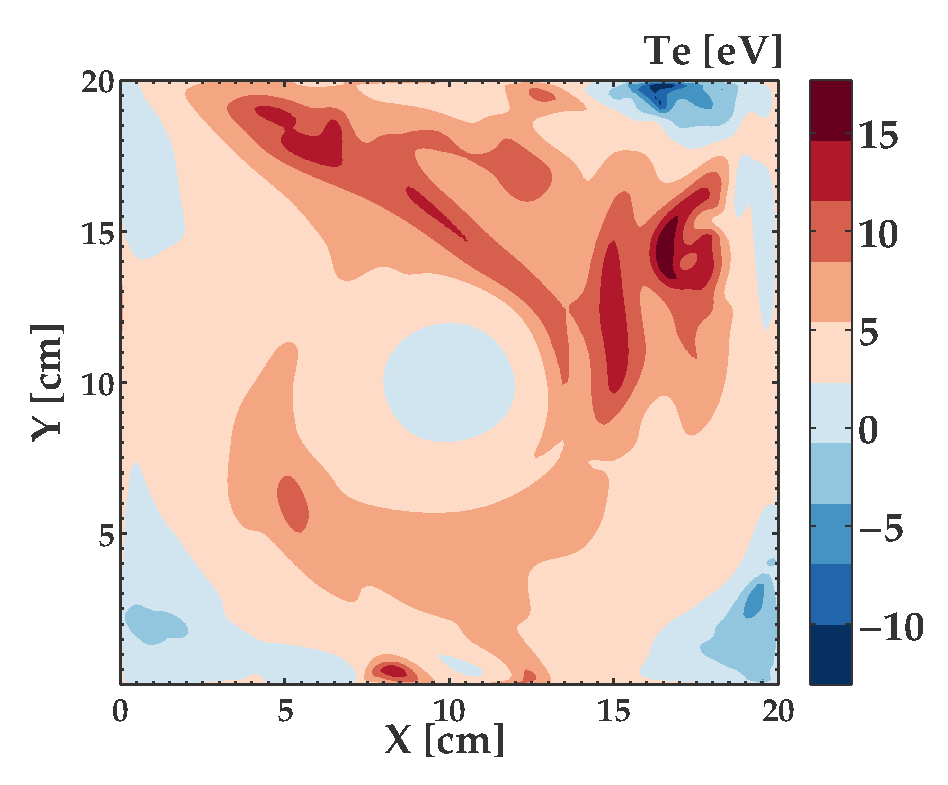
\includegraphics[width=0.8\textwidth]{figures/4-CybeleCartePhiSurTeBase.eps}
{\caption{Carte du potentiel électrostatique rapporté à la température
électronique.}
\label{4-CybeleCartePhiSurTeBase}}
\end{figure}

a

\begin{figure}[htbp]
  \centering
    \subfigure[]{\label{4-CybeleCarteFluxIBase}
    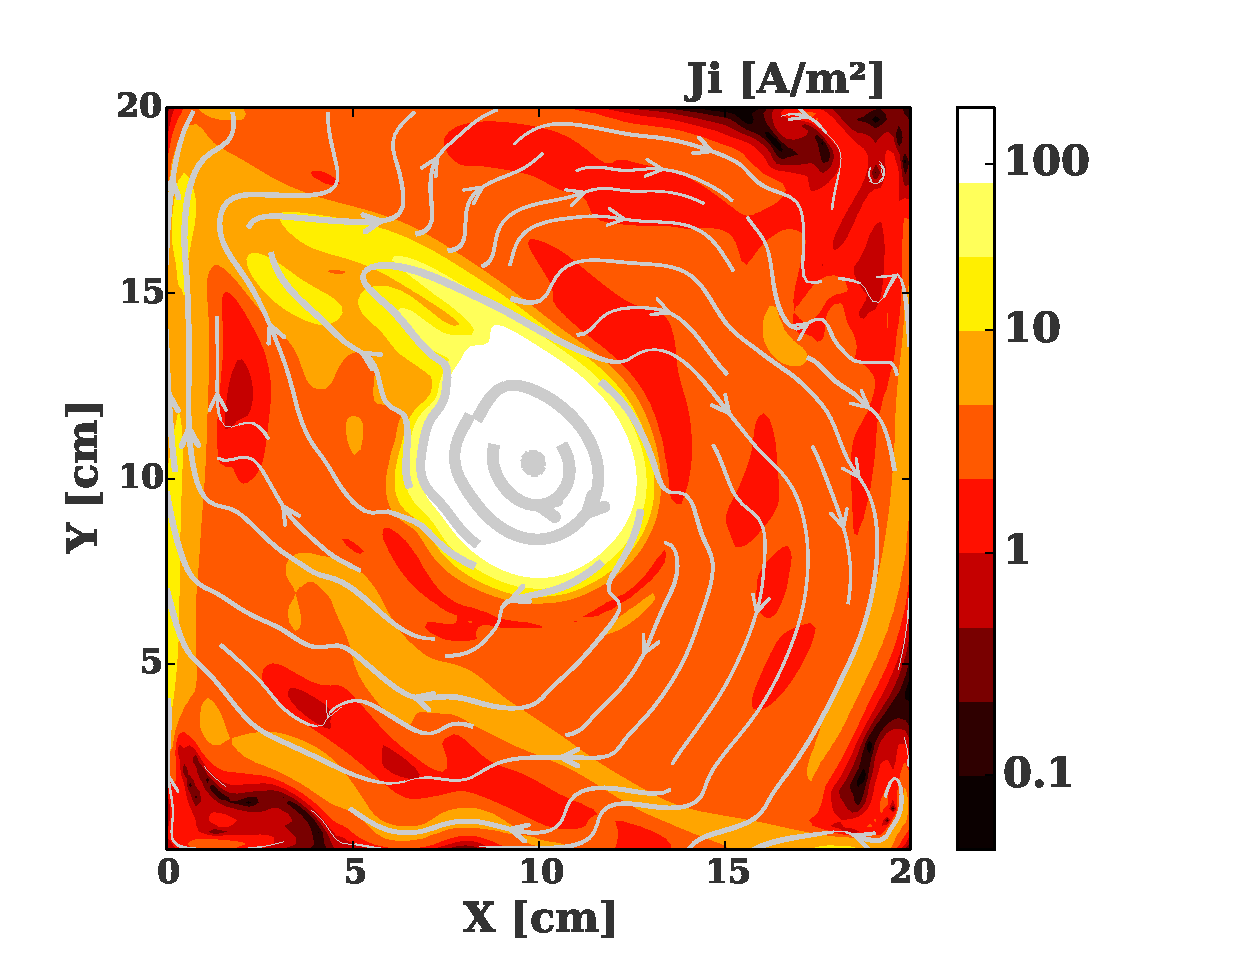
\includegraphics[height=5.5cm]{figures/4-CybeleCarteFluxIBase.eps}}
    \subfigure[]{\label{4-CybeleCarteFluxEBase}
    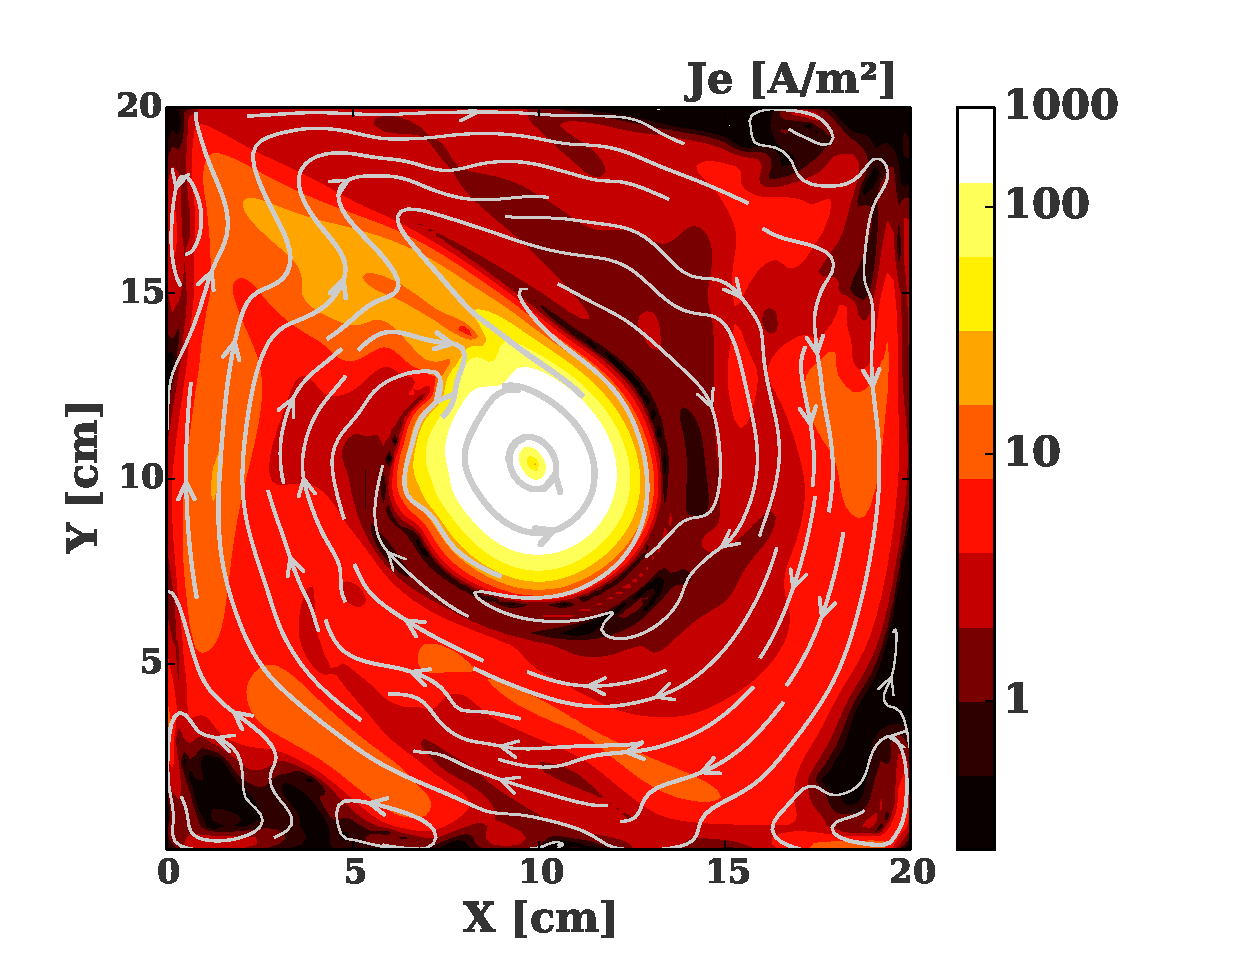
\includegraphics[height=5.5cm]{figures/4-CybeleCarteFluxEBase.eps}}
    \caption{Cartes de densité \subref{4-CybeleCarteFluxEBase}~ et de
    température \subref{4-CybeleCarteCourant}}
    \label{pandas}
\end{figure}

a

\subsection{Le transport transverse magnétisé}

\begin{figure}[htbp]
  \centering
    \subfigure[]{\label{4-CybeleVarMag1}
    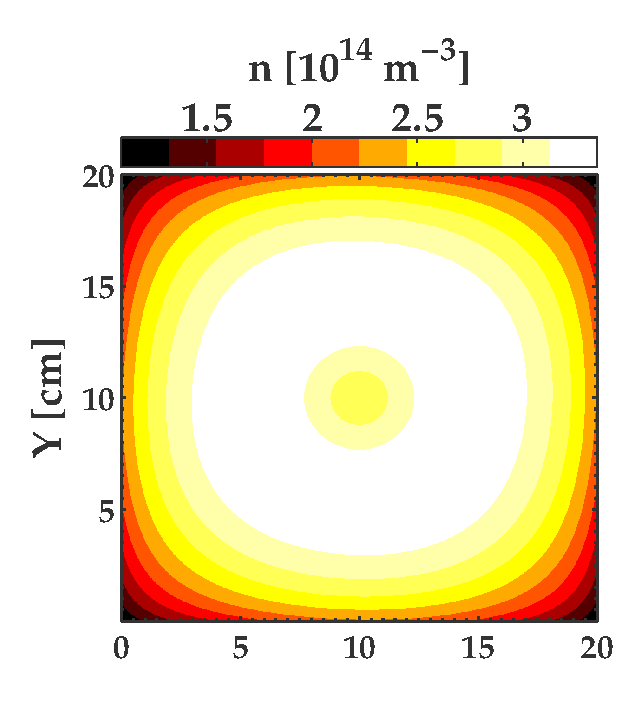
\includegraphics[height=5.5cm]{figures/4-CybeleVarMag1.eps}}
    \subfigure[]{\label{4-CybeleVarMag2}
    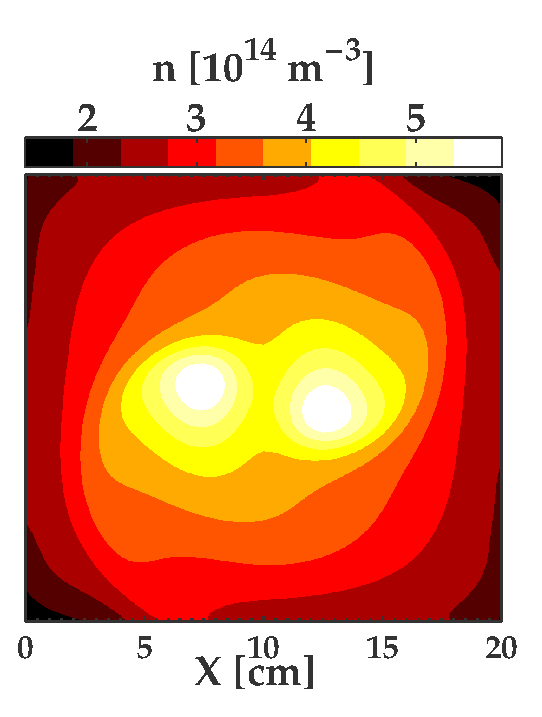
\includegraphics[height=5.5cm]{figures/4-CybeleVarMag2.eps}}
    \subfigure[]{\label{4-CybeleVarMag3}
    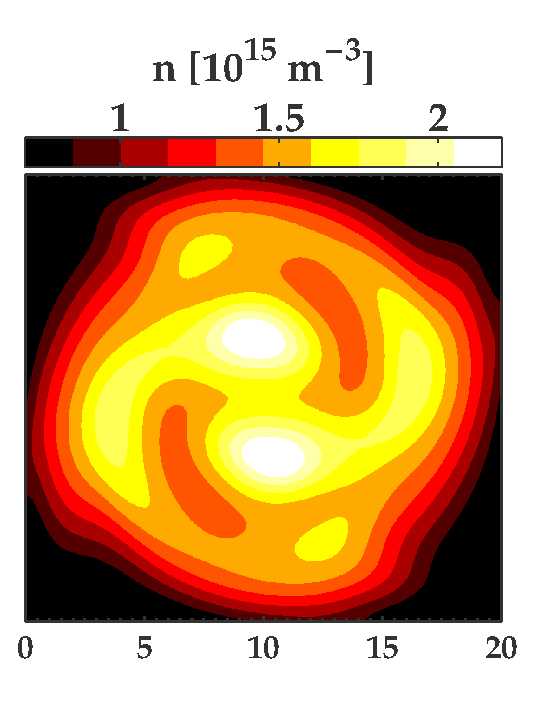
\includegraphics[height=5.5cm]{figures/4-CybeleVarMag3.eps}}
    \caption{Cartes de densité à 1G\subref{4-CybeleVarMag1}~, 4G
    \subref{4-CybeleVarMag2}~ et 15G \subref{4-CybeleVarMag3}}
    \label{pandas}
\end{figure}

a

\begin{figure}[htbp]
  \centering
    \subfigure[]{\label{4-CybeleVarMag4}
    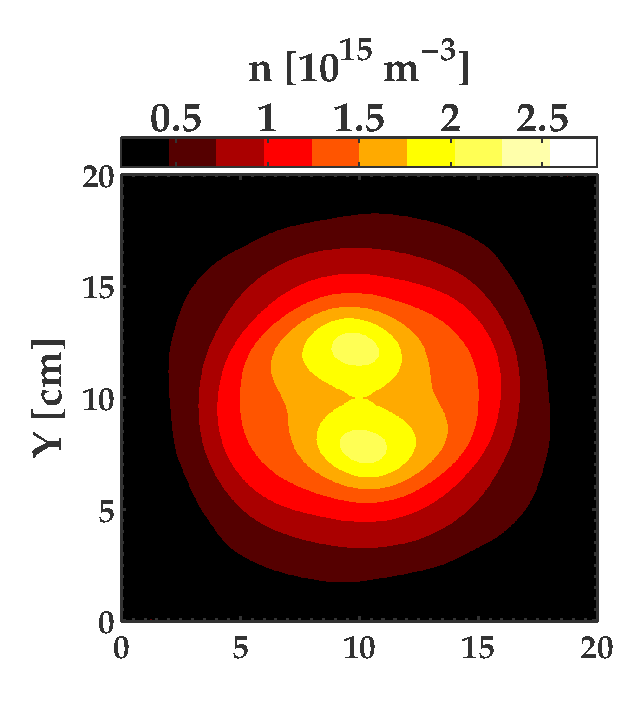
\includegraphics[height=5.5cm]{figures/4-CybeleVarMag4.eps}}
    \subfigure[]{\label{4-CybeleVarMag5}
    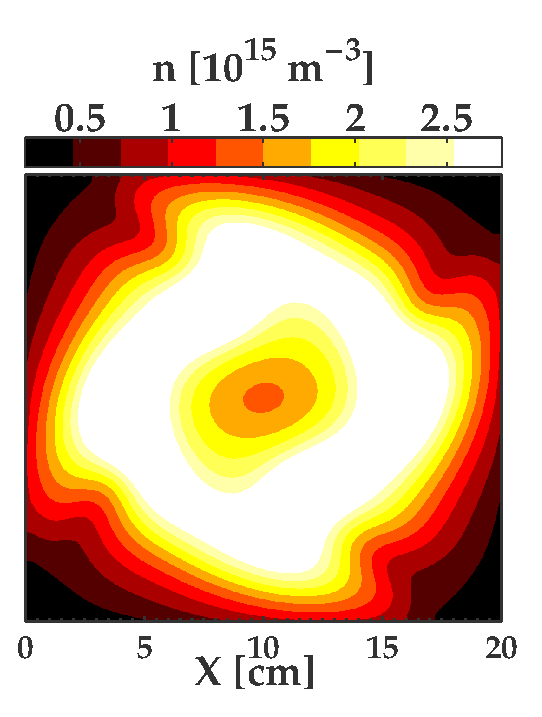
\includegraphics[height=5.5cm]{figures/4-CybeleVarMag5.eps}}
    \subfigure[]{\label{4-CybeleVarMag6}
    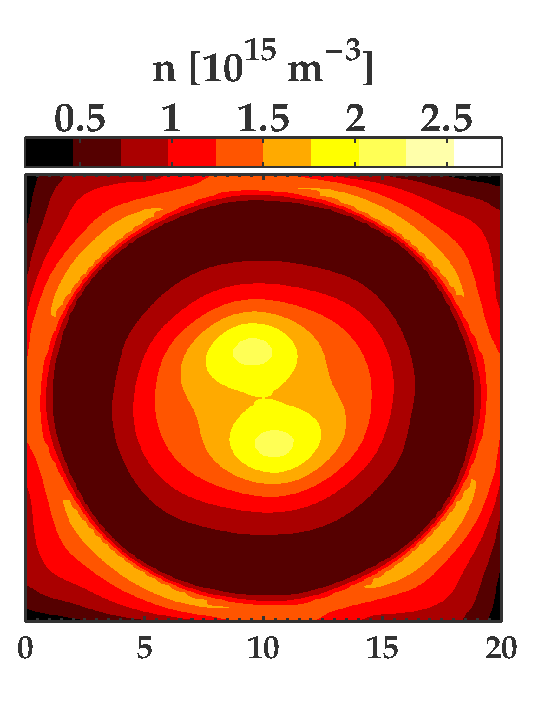
\includegraphics[height=5.5cm]{figures/4-CybeleVarMag6.eps}}
    \caption{Cartes de densité à 20G\subref{4-CybeleVarMag4}~, de
    potentiel \subref{4-CybeleVarMag5}~ et de
    température \subref{4-CybeleVarMag6}}
    \label{pandas}
\end{figure}

a

\begin{figure}[htbp]
\centering
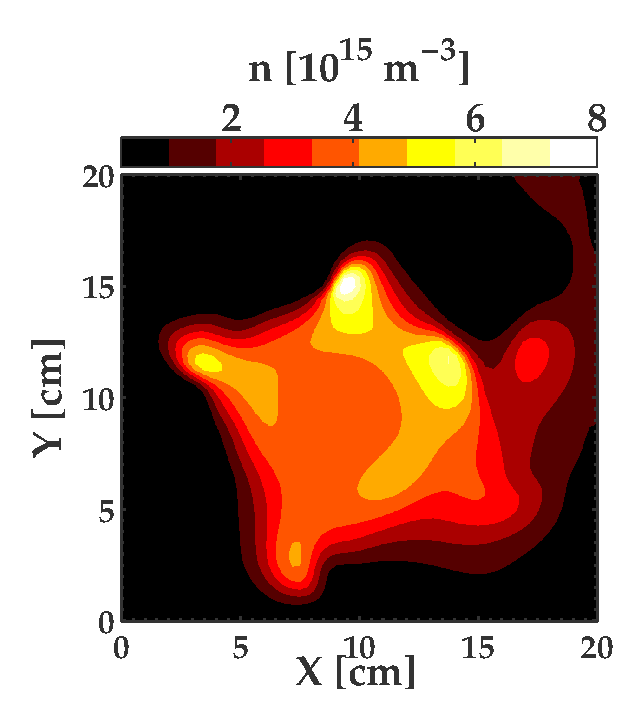
\includegraphics[width=0.5\textwidth]{figures/4-CybeleVarMag8.eps}
{\caption{Carte de densité à 35G.}
\label{4-CybeleVarMag8}}
\end{figure}

a

\begin{figure}[htbp]
  \centering
    \subfigure[]{\label{4-CybeleVarMag9}
    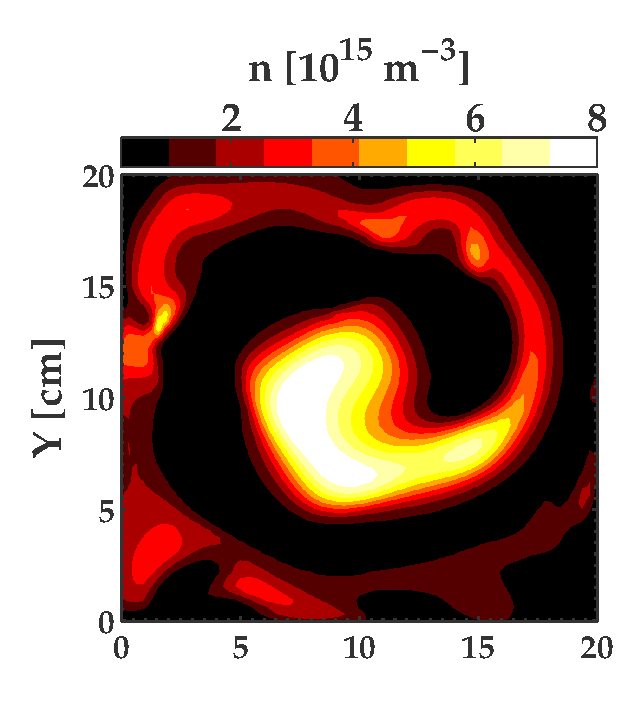
\includegraphics[height=5.5cm]{figures/4-CybeleVarMag9.eps}}
    \subfigure[]{\label{4-CybeleVarMag10}
    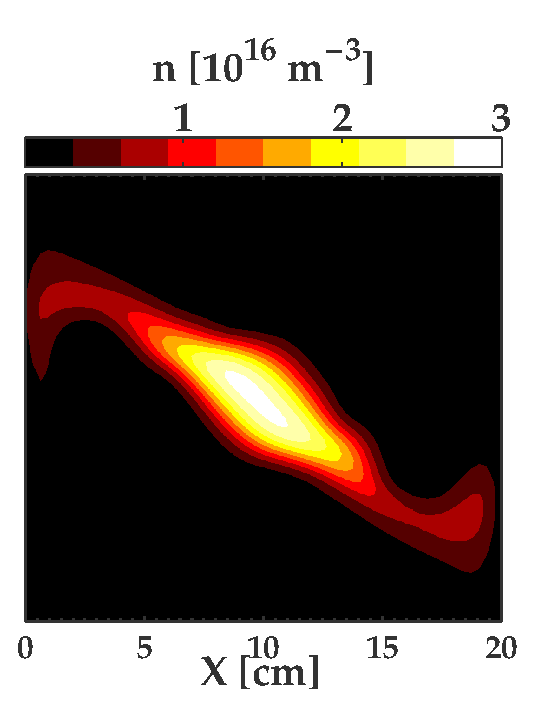
\includegraphics[height=5.5cm]{figures/4-CybeleVarMag10.eps}}
    \subfigure[]{\label{4-CybeleVarMag11}
    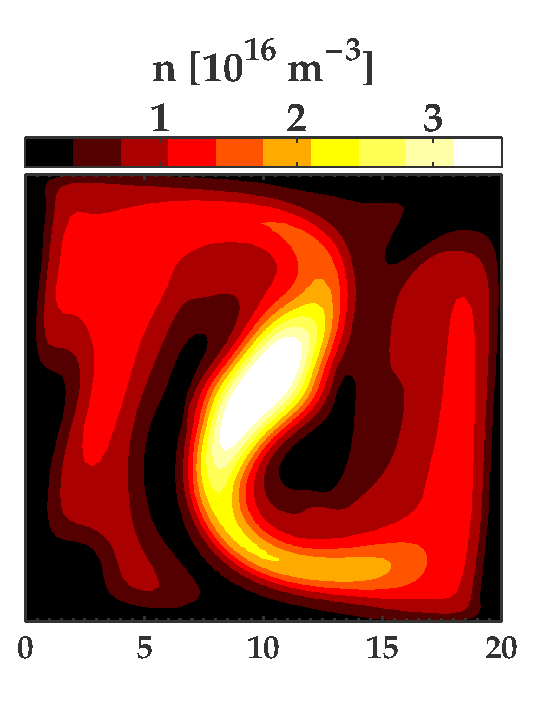
\includegraphics[height=5.5cm]{figures/4-CybeleVarMag11.eps}}
    \caption{Cartes de densité à 80G\subref{4-CybeleVarMag9}~, 130G
    \subref{4-CybeleVarMag10}~ et 170G \subref{4-CybeleVarMag11}}
    \label{pandas}
\end{figure}

a
\begin{table*}
\footnotesize\centering
\ra{1.3}
\begin{tabular}{@{}cccccccccc@{}}\toprule
B&&\multicolumn{3}{c}{Echelles} && \multicolumn{2}{c}{Champs} &&
Rotation\\
\cmidrule{3-5} \cmidrule{7-8} \cmidrule{10-10}
&& $\omega_c$ & $\rho\indice{L}$& $l_{\text{lpm}}$&& $n$ & $T_e$ && 
$\Omega_r$\\
\midrule Phase 1\\
\scriptsize 1-15 &&\scriptsize 10\textsuperscript{4} - 2 10\textsuperscript{5} &
\scriptsize0.1692 &\scriptsize 0.2945 && \scriptsize0.3670 &\scriptsize 0.7187
&& \scriptsize3.1815 \\
Phase 2\\
\scriptsize1-15 &&\scriptsize 10\textsuperscript{4} - 2 10\textsuperscript{5} &
\scriptsize0.1692 &\scriptsize 0.2945 &&\scriptsize 0.3670 &\scriptsize 0.7187
&&\scriptsize 3.1815 \\
Phase 3\\
\scriptsize1-15 &&\scriptsize 10\textsuperscript{4} - 2 10\textsuperscript{5} &
\scriptsize0.1692 &\scriptsize 0.2945 &&\scriptsize 0.3670 &\scriptsize 0.7187
&&\scriptsize 3.1815 \\

\bottomrule
\end{tabular}
\caption{Caption}
\end{table*}
	
	\subsection{Influence du champ magnétique}
	\subsubsection{Influence de la densité de gaz}
\subsection{Polarisation des parois}
		

\section{Plasma de bord de tokamaks}
%\bibliographystyle{apalike}
%\bibliography{biblio}
\end{refsection}
